\section{Гипербола}
\begin{wrapfigure}[19]{r}{0pt}\noindent
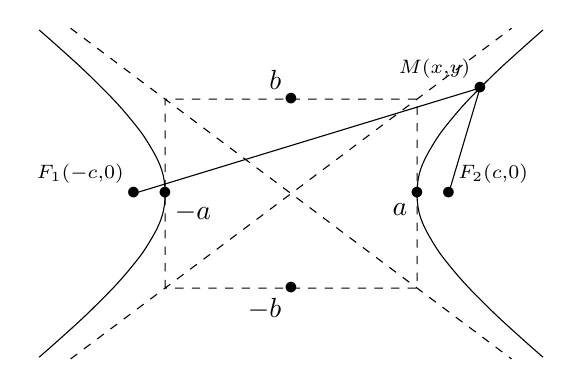
\begin{tikzpicture}[scale=0.4]
\drawaxis{-8}{8}{-5}{5};

% рисуем гиперболу x^2/16 - y^2/9 = 1
\draw (-5, 0) coordinate (F1) node {$\bullet$} node[above left] {$\scriptstyle F_1(-c, 0)$}
	(5, 0) coordinate (F2) node {$\bullet$} node[above right] {$\scriptstyle F_2(c, 0)$}
	(6, 3.3541) coordinate (M) node {$\bullet$} node [above left] {$\scriptstyle M(x, y)$}
	-- (F1) (M) -- (F2);
\def\painthyperbola[#1]{
\draw[#1] (4, 0)
	to[out=90, in=-121] (4.5, 1.5462)
	to[out=59, in=-129] (5, 9/4)
	to[out=51, in=-135] (6, 3.3541)
	to[out=45, in=-138] (7, 4.3084)
	to[out=42, in=-139] (8, 5.1962)
}
\painthyperbola[];
\painthyperbola[xscale=-1];
\painthyperbola[yscale=-1];
\painthyperbola[xscale=-1, yscale=-1];

% рисуем асимптоты
\draw[dashed] (-4, -3) rectangle (4, 3)
	(-7, 5.25) -- (7, -5.25)
	(-7, -5.25) -- (7, 5.25)
	(-4, 0) node {$\bullet$} node[below right] {$-a$}
	(4, 0) node {$\bullet$} node[below left] {$a$}
	(0, -3) node {$\bullet$} node[below left] {$-b$}
	(0, 3) node {$\bullet$} node[above left] {$b$};
\end{tikzpicture}
\end{wrapfigure}

\index{Гипербола} \textbf{Гиперболой} называется геометрическое место точек~$M$ таких, что $|MF_1 - MF_2| = 2a < F_1 F_2$, где $a$~--- константа, $F_1$ и $F_2$~--- фиксированные точки, называемые \textbf{фокусами гиперболы}.

Пусть $F_1 = (-c, 0)$, $F_2 = (c, 0)$, $M = (x, y)$.
Найдём уравнение гиперболы.
\begin{equation*}
\left|\sqrt{(x + c)^2 + y^2} - \sqrt{(x - c)^2 + y^2}\right| = 2a \Rightarrow
\end{equation*}
\begin{equation*}
\Rightarrow 2x^2 + 2y^2 + 2c^2 - 2\sqrt{(x^2 + y^2 + c^2)^2 - 4c^2 x^2} = 4a^2 \Rightarrow
\end{equation*}
\begin{equation*}
\Rightarrow (2a^2 - (x^2 + y^2 + c^2))^2 = (x^2 + y^2 + c^2)^2 - 4c^2 x^2 \Leftrightarrow
\end{equation*}
\begin{equation*}
\Leftrightarrow a^4 - a^2 x^2 - a^2 y^2 - a^2 c^2`+ c^2 x^2 = 0 \Leftrightarrow
\end{equation*}
\begin{equation*}
\Leftrightarrow (a^2 - c^2) x^2 + a^2 y^2 = a^2 (a^2 - c^2) \Leftrightarrow
\end{equation*}
\begin{equation*}
\left|\text{Пусть $b^2 = c^2 - a^2$}\right|
\Leftrightarrow -b^2 x^2 + a^2 y^2 = -a^2 b^2 \Leftrightarrow
\frac{x^2}{a^2} - \frac{y^2}{b^2} = 1
\end{equation*}

\subsection{Уравнение касательной}
Найдём уравнение касательной, проходящей через точку~$(x_0, y_0)$ гиперболы.
\begin{equation*}
y = \pm b\,\sqrt{\frac{x^2}{a^2} - 1} \Rightarrow
y' = \pm\frac{ab}{2\sqrt{x^2 - a^2}} \cdot \frac{2x}{a^2} =
\pm\frac{bx}{a\sqrt{x^2 - a^2}} \;
\left|y = \pm b\,\sqrt{\frac{x^2}{a^2} - 1} \Leftrightarrow
\sqrt{x^2 - a^2} = \pm\frac{a}b\,y\right| =
\frac{b^2 x}{a^2 y}
\end{equation*}
\begin{equation*}
y = y_0 + \frac{b^2 x_0}{a^2 y_0} (x - x_0) \Leftrightarrow
a^2 (y - y_0) y_0 = b^2 (x - x_0) x_0 \Leftrightarrow
\frac{x x_0}{a^2} - \frac{y y_0}{b^2} - \left(\frac{x_0^2}{a^2} - \frac{y_0^2}{b^2} \right) = 0 \Leftrightarrow
\frac{x x_0}{a^2} - \frac{y y_0}{b^2} = 0
\end{equation*}

\subsection{Асимптоты}
Докажем, что прямые~$y = \pm\frac{b}a\,x$~--- асимптоты гиперболы.
Пусть точка~$M(x, y)$ лежит на гиперболе, где $y > 0$, а точка~$N(x, Y)$~--- на прямой~$y = \frac{b}a\,x$.
Тогда
\begin{equation*}
MN = \frac{b}a \left(x - \sqrt{x^2 - a^2}\right) =
\frac{ab}{x + \sqrt{x^2 - a^2}} \Rightarrow
\lim_{x \to +\infty} MN =
\lim_{x \to +\infty} \frac{ab}{x + \sqrt{x^2 - a^2}} = 0
\end{equation*}

Рсстояние~$MN$ стремится к нулю при возрастании абсциссы, значит, $y = \frac{b}a\,x$~--- асимптота гиперболы.

Аналогично доказывается для случая~$y < 0$ и для прямой~$y = -\frac{b}a\,x$.